%!TEX encoding = UTF-8
% --build requirements-------------------
% |	command	: uplatex					|
% |	Fonts	: NotoSansCJKjp				|
% |			  NotoSerifCJKjp			|
% ---------------------------------------
\documentclass[uplatex]{jsarticle}
\usepackage[dvipdfmx]{graphicx}

\usepackage{siunitx}		%for use si unit
\usepackage{here}			%for use figure here
\usepackage{tikz}			%for use TikZ package
\usepackage{pgfplots}		%for use PGFplots
\usepackage{dcolumn}		%for use significant figures in the table
\usepackage{csvsimple}		%for import csv files
\usepackage[RPvoltages,europeanresistors,americaninductors,europeanvoltage,americancurrents]{circuitikz}

\usepackage[noto]{pxchfon}	%for use Noto fonts

\usepackage{bxtexlogo}
\bxtexlogoimport{TikZ}

\tikzset{% tikz style set
  	pointtype triangle/.style={mark=triangle*,mark size=4pt},
  	every mark/.style={fill=white,solid},
  	south west label/.style={
		matrix,matrix of nodes,
		anchor=south west,at={(rel axis cs:0.01,0.01)},
		nodes={anchor=west,inner sep=0},
  	},
}

\pgfplotsset{% graph style set
    table/col sep=comma, % Use CSV files
  	compat=1.12,
  	major tick length=0.2cm,
  	minor tick length=0.1cm,
  	every axis/.style={semithick},
  	tick style={semithick,black},
  	legend cell align=left,
  	legend image code/.code={%
		\draw[mark repeat=2,mark phase=2,#1]
	  	plot coordinates {(0cm,0cm) (0.5cm,0cm) (1.0cm,0cm)};
  	},
  	log number format basis/.code 2 args={
	\pgfmathsetmacro\e{#2}
	\pgfmathparse{#2==0}\ifnum\pgfmathresult>0{1}\else
	\pgfmathparse{#2==1}\ifnum\pgfmathresult>0{10}\else
	{$#1^{\pgfmathprintnumber{\e}}$}\fi\fi},
}

\title{高専低学年向けの\LaTeX 教材の提案}
\author{Takahiro TOKANO}
\date{\today}

\begin{document}

\maketitle

\section{はじめに}
	本学では各学科2~3年からレポート課題が課される傾向がある。
	近年では手書きでなくPCで作成したものでの提出を許可する教員も多いが、
	PCでレポートを書く方法に関してはフォーマットに関する指導のみで作成方法についてはほとんど指導がない\footnote{電子制御工学科学生による情報}。
	このため多くの学生がレポートをすべて手書きで作成しているか、
	適切なソフトを用いておらず低品位なレポートが作成されているのが実情である。

	この低学年の実情を踏まえ、PCでのレポート作成に関する教材を制作することを提案したい。
	また、高専卒業後進学する学生もいることを踏まえ、電気情報分野の論文執筆に大きなシェアを持つ\LaTeX
	を題材として教材を作成することとする。

	本教材では、\LaTeX の執筆技術への深い理解は大きな目的とせず、
	高専低学年で高品位なレポートを作成する方法を習得し、
	高学年や進学時での論文執筆へ活用することを第一の目的とする。

\section{概要}
	\LaTeX を一度も使ったことない読者を想定するものとし、以下の内容を盛り込むものとする。

	% \begin{itemize}
	% 	\item \LaTeX の成り立ちや動作原理の解説
	% 	\item 環境構築
	% 	\item 文書作成の方法
	% 	\item 実験データの取り方
	% 	\item 図表作成の方法
	% 	\item Gitによるバージョン管理法
	% \end{itemize}

	\subsection{\LaTeX の成り立ちや動作原理の解説}
		この章では、\LaTeX とは何かを解説する。
		なぜMicrosoft WordのようなWYSIWYG形式でなく一見煩わしいマークアップ言語による記述を用いるのか、
		\TeX と\LaTeX の成り立ちや動作原理などを簡単かつ必要最小限に説明する。

	\subsection{環境構築}
		\TeX ディストリビューションとして最もポピュラーな\TeX Liveを使用するものとし、
		エディタは執筆用の拡張機能やGitとの連携が強力であり、
		初学者にもわかりやすいGUIを備えた
		Microsoft Visual Studio Codeを使用することとし環境構築を解説する。

	\subsection{文書作成の方法}
		\LaTeX の文書構造、章立ての方法、図表の挿入等一般的な執筆方法に関して解説する。

	\subsection{グラフの生成}
		レポートの作成にはグラフの生成が必要不可欠であるが、現在無料で使用できるグラフソフトは限られており、
		GUIを持つものとして代表的なNgraphは開発が停止しており\footnote{Windows向けビルドの最終更新は2015年である}
		CLI形式として代表的なgnuplotもあるが初学者には難解であり、本教材には向かない。

		そこで、\LaTeX でグラフを生成できるPGFPlots\footnote{対してPGFPlotsは執筆時点で4日前に更新されている}を取り扱うこととする。
		PGFPlotsは、gnuplotより簡単な構文で論文レベルの高品位なグラフを生成することが可能である。
		また\LaTeX 構文上でグラフの描画命令を記述でき、ビルド毎にグラフが生成されるため、
		他のソフトで一度PDF形式などに出力する煩雑な手間を省くことが可能であり、修正なども容易になる。
		例として以下の図\ref{fig:XLXC}に
		RL直列回路の誘導性リアクタンス及びRC直列回路の容量性リアクタンスをプロットしたグラフを示す。

		\begin{figure}[H]
			\centering
			\begin{tikzpicture}
				\begin{axis}[
					width=100mm, height=100mm,
					xmin = 0 , xmax = 109,
					ymin = 0 , ymax = 800,
					xlabel={周波数[\si{\kilo\hertz}]},
					ylabel={リアクタンス[\si{\ohm}]},
					legend entries={誘導性リアクタンス,容量性リアクタンス},
					legend style={at={(1,1)},anchor=north east}
					]
					\addplot[mark=*,only marks] table {data1.csv};
					\addplot[mark=square*,only marks] table {data2.csv};

					\addplot[mark=none,domain=0:110,samples=100] {2*3.14*x};
					\addplot[mark=none,domain=0:110,samples=100] {1/(x*2*3.14*0.022*0.001)};
				\end{axis}
			\end{tikzpicture}
			\caption{周波数とリアクタンスの関係}
			\label{fig:XLXC}
		\end{figure}

		このグラフでは、実際に実験で計測したデータをCSVで保存したものをPGFPlotsに入力し実験値の点をプロットしている。
		このような実験データの管理方法も解説する。

    \subsection{回路図の生成}
        電気系学科では欠かせない回路図であるが、
        レポートや論文に用いることができる高品位な回路図の生成は一般的なCADで生成することが難しい。
        一般的な回路図CADであるKiCadを用いて生成したRL直列回路の回路図を図\ref{fig:kicad-circuit}に示す。

		\begin{figure}[H]
			\centering
			\begin{tabular}{c}
				\begin{minipage}{0.50\hsize}
					\centering
					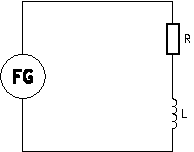
\includegraphics[width=4cm]{circuit.pdf}
					\caption{KiCadで生成した回路図}
					\label{fig:kicad-circuit}
                \end{minipage}
                
                \begin{minipage}{0.50\hsize}
					\centering
					\begin{circuitikz}[scale=1.5]
						\draw (0,0)
						to[sV,l=$FG$] (0,2);
						\draw (0,2)
						to[short] (2,2);
						\draw (2,2)
						to[R,l_=$R$] (2,1);
						\draw (2,1)
						to[L,l_=$L$] (2,0);
						\draw (2,0)
						to[short] (0,0);
					\end{circuitikz}
					\caption{Circui{\TikZ}で生成した回路図}
					\label{fig:circuitikz-circuit}
				\end{minipage}
			\end{tabular}
        \end{figure}
        
        そこで、\LaTeX で回路図を生成できるCircui{\TikZ}を取り扱うこととする。
        図\ref{fig:circuitikz-circuit}にCircui{\TikZ}で生成したRL直列回路の回路図を示す。
        \LaTeX 構文上で回路図を生成できるので、再度編集する際も容易である。

\end{document}